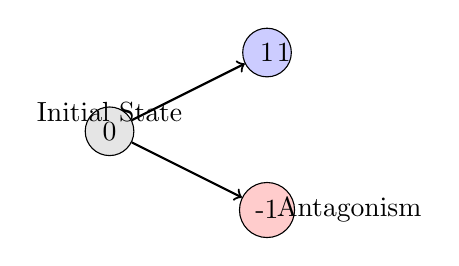
\begin{tikzpicture}
\node[circle, draw, fill=gray!20] at (0,0) (O) {0};
\node[circle, draw, fill=blue!20] at (2,1) (P1) {1};
\node[circle, draw, fill=red!20] at (2,-1) (M1) {-1};
\draw[->, thick] (O) -- node[above] {$\Opp$} (P1);
\draw[->, thick] (O) -- node[below] {$\Opp$} (M1);
\node[above] at (O) {Initial State};
\node[right] at (P1) {$\F{1}$};
\node[right] at (M1) {Antagonism};
\end{tikzpicture}
